\begin{figure}
  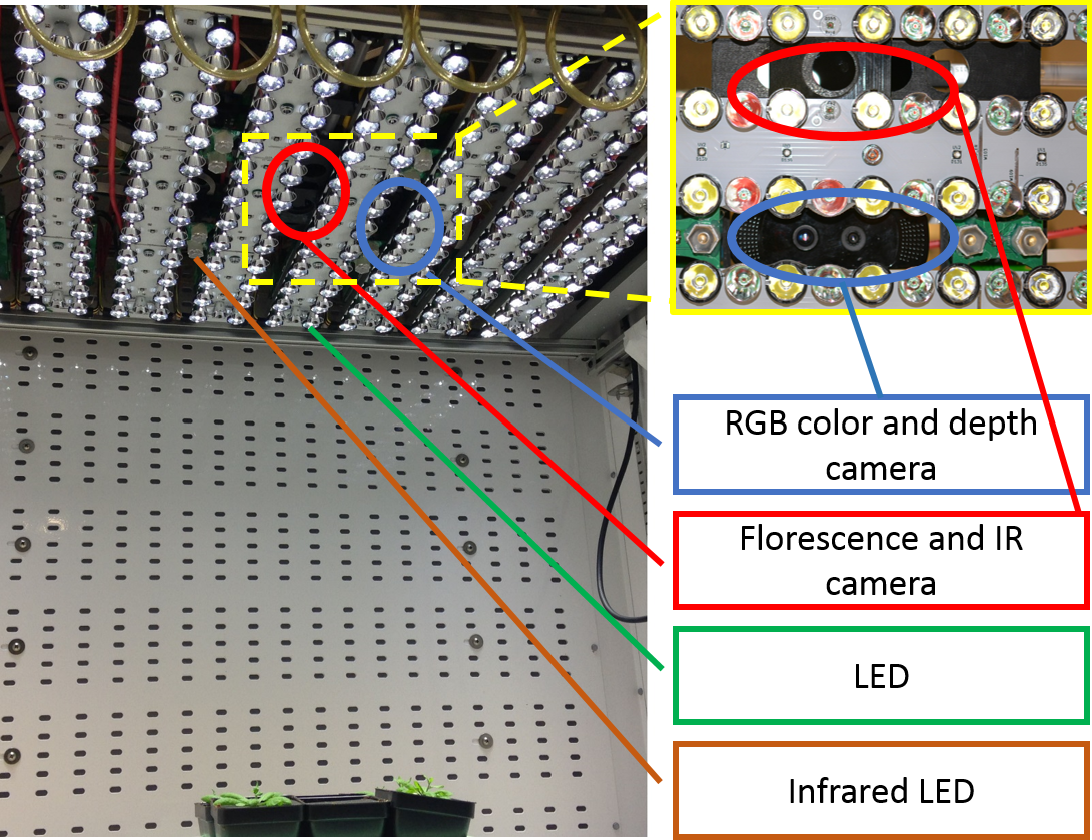
\includegraphics[width=\linewidth,trim=55 100 200 70,clip]{Figures/hardware}
\caption{The hardware setup for our data collection.}
\label{fig:hardware}
\end{figure}

\subsection{Hardware Setup}

In this section, we introduce the hardware used for capturing fluorescence, IR, RGB color, and depth imagery data for both plants.
Figure~\ref{fig:hardware} illustrates the hardware and imaging setup used in our data collection.

\subsubsection{Fluorescence and IR images}
Chlorophyll a fluorescence images were captured once every hour during the daylight period in a growth chamber~\cite{cruz2015depi}.
A set of $5$ images were captured using a Hitachi KP-F145GV CCD camera (Hitachi Kokusai Electric America Inc., Woodbury, NY) outfitted with an infrared long pass filter (Schott Glass RG-9, Thorlabs, Newton, NJ), during a short period ($<400~ms$) of intense light saturating to photosynthesis ($>10,000~\mu mol~photons~m^{-2} s^{-1}$) provided by an array of white Cree LEDs (XMLAWT, 5700K color temperature, Digi-Key, Thief River Falls, MN) collimated using a $20~mm$ Carclo Lens (10003, LED Supply, Lakewood, CO).
%
Chlorophyll a fluorescence was excited using monochromatic red LEDs (Everlight $625~nm$, ELSH-F51R1-0LPNM-AR5R6, Digi-Key), collimated using a Ledil reflector optic ($C11347\_REGINA$, Mouser Electronics, Mansfield, TX) and pulsed for $50~\mu s$ during a brief window when the white LEDs were electronically shuttered.
In addition, a series of $5$ images were also collected in the absence of the excitation light for artifact subtraction.

Infrared images were collected once every hour with the same camera and filter used for chlorophyll a fluorescence.
Pulses of $940~nm$ light were provided by an array of OSRAM LEDs (SFH 4239, Digi-Key), collimated using a Polymer Optics lens (Part no. 170, Polymer Optics Ltd., Berkshire, England).
Since $940~nm$ light does not influence plant development or drive photosynthesis, images were also collected during the night period.
Sets of $15$ images were collected for averaging, in the absence of saturating illumination.
As with chlorophyll a fluorescence, images were captured in the absence of $940~nm$ light for artifact subtraction.



\subsubsection{RGB color and depth images} %This section describes characterizes the data from this sensor, particularly the depth data.

The RGB color and depth images were collected using a Creative Senz3D sensor~\cite{nguyen2015vietnamese}. The sensor contains both a $1280 \times 720$ color camera directed parallel to, and separated by roughly $25~mm$ from, a depth camera which has a resolution of $320\times240$ pixels.
The depth sensor uses a flash near IR illuminator and measures the time-of-flight of the beam at each pixel to obtain dense depth estimates along with an IR reflectance at each pixel.

There are a number of limitations to the depth sensor that become the sources of depth errors.
The primary measurement limitation on the range-to-target is the strength of the reflected beam.
As a result, dark, matt surfaces are measured reliably only at a close range on the order of $20$ or $30~cm$.
Highly reflective surfaces also pose problems with direct reflections leading to saturation and highly unreliable depths.
In addition reflective surfaces at grazing angles are less reliably measured since little signal is reflected.
Fortunately the primary goal of the depth measurements are to obtain leaf depths, and plants provide good, roughly Lambertian, reflections of IR~\cite{Chelle2006219}.  Thus the depth pixels that are most reliable and are of most use are those that fall on plant foliage.

% For one-column wide figures use
\begin{figure}
\begin{tabular}{c}
  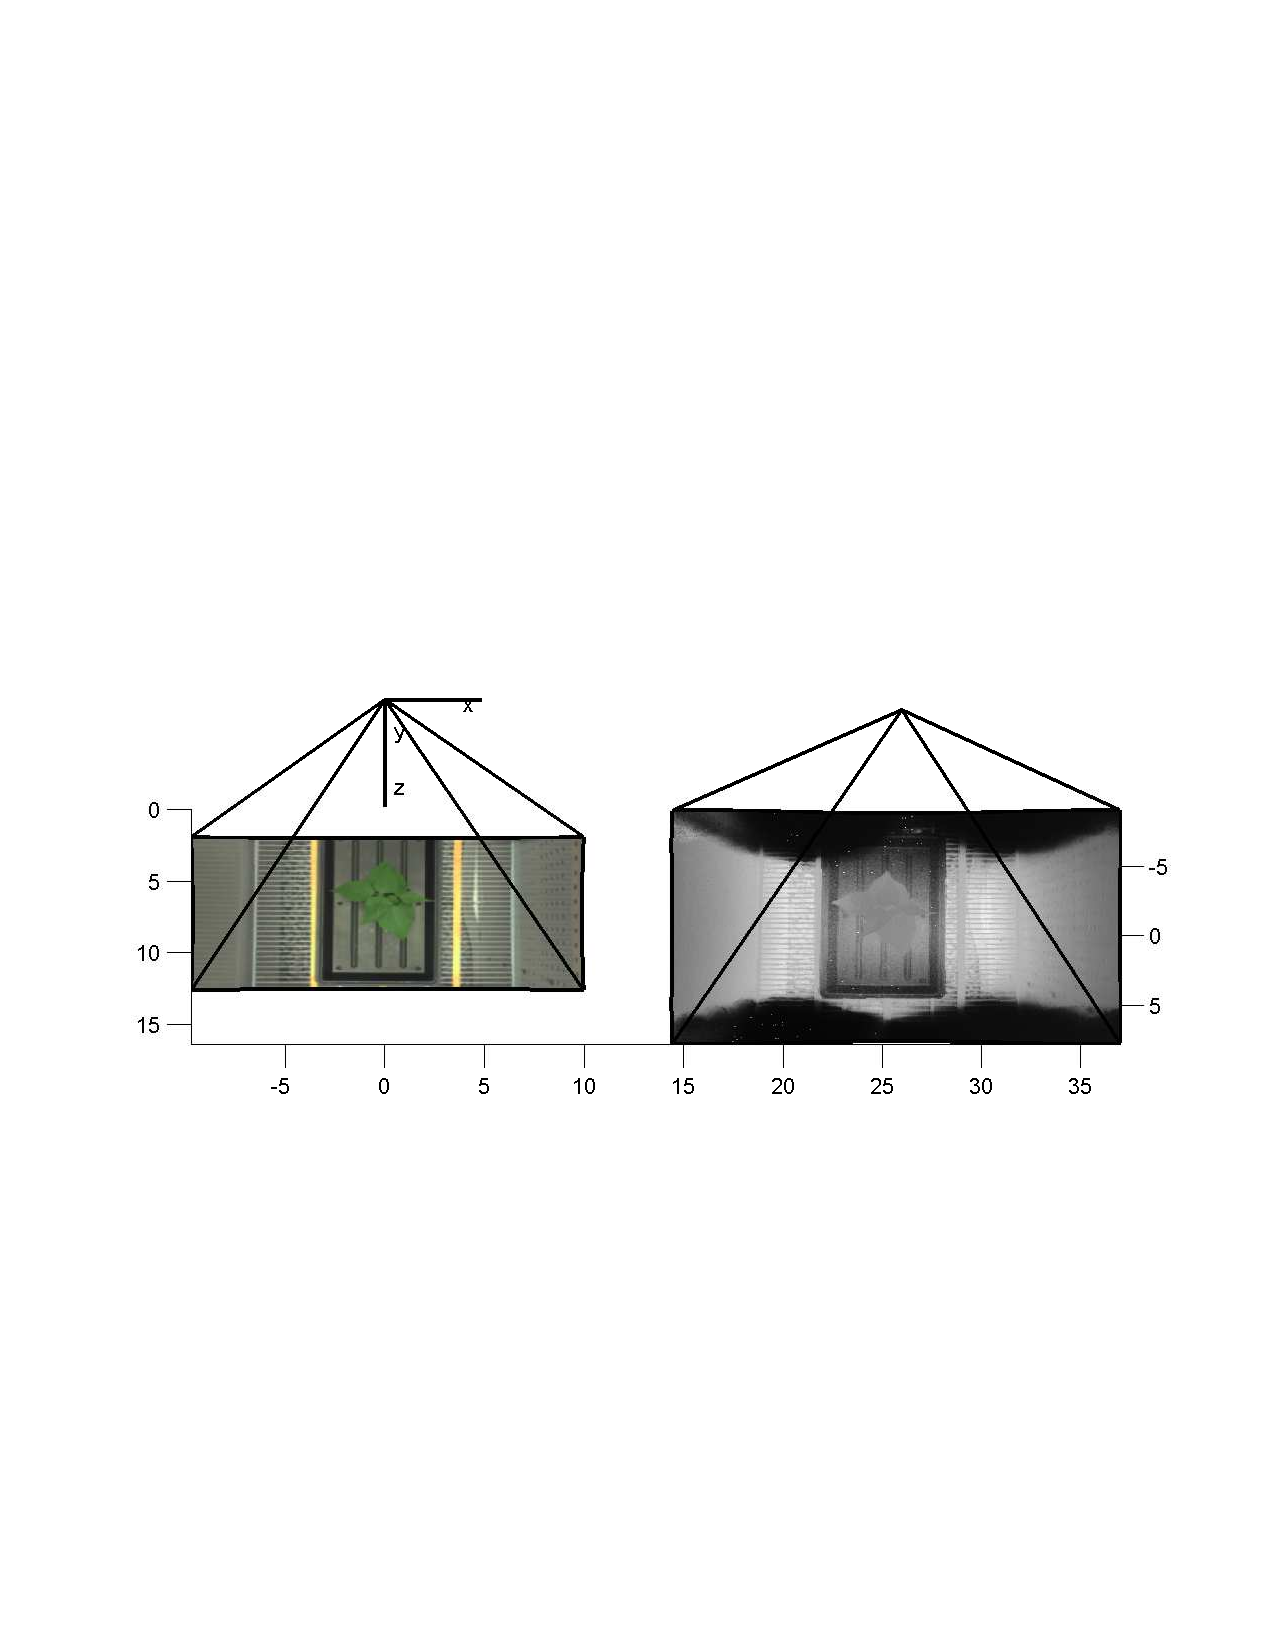
\includegraphics[width=\linewidth,trim=120 240 80 300,clip]{Figures/CameraConfiguration} \\
  ($a$)\\
  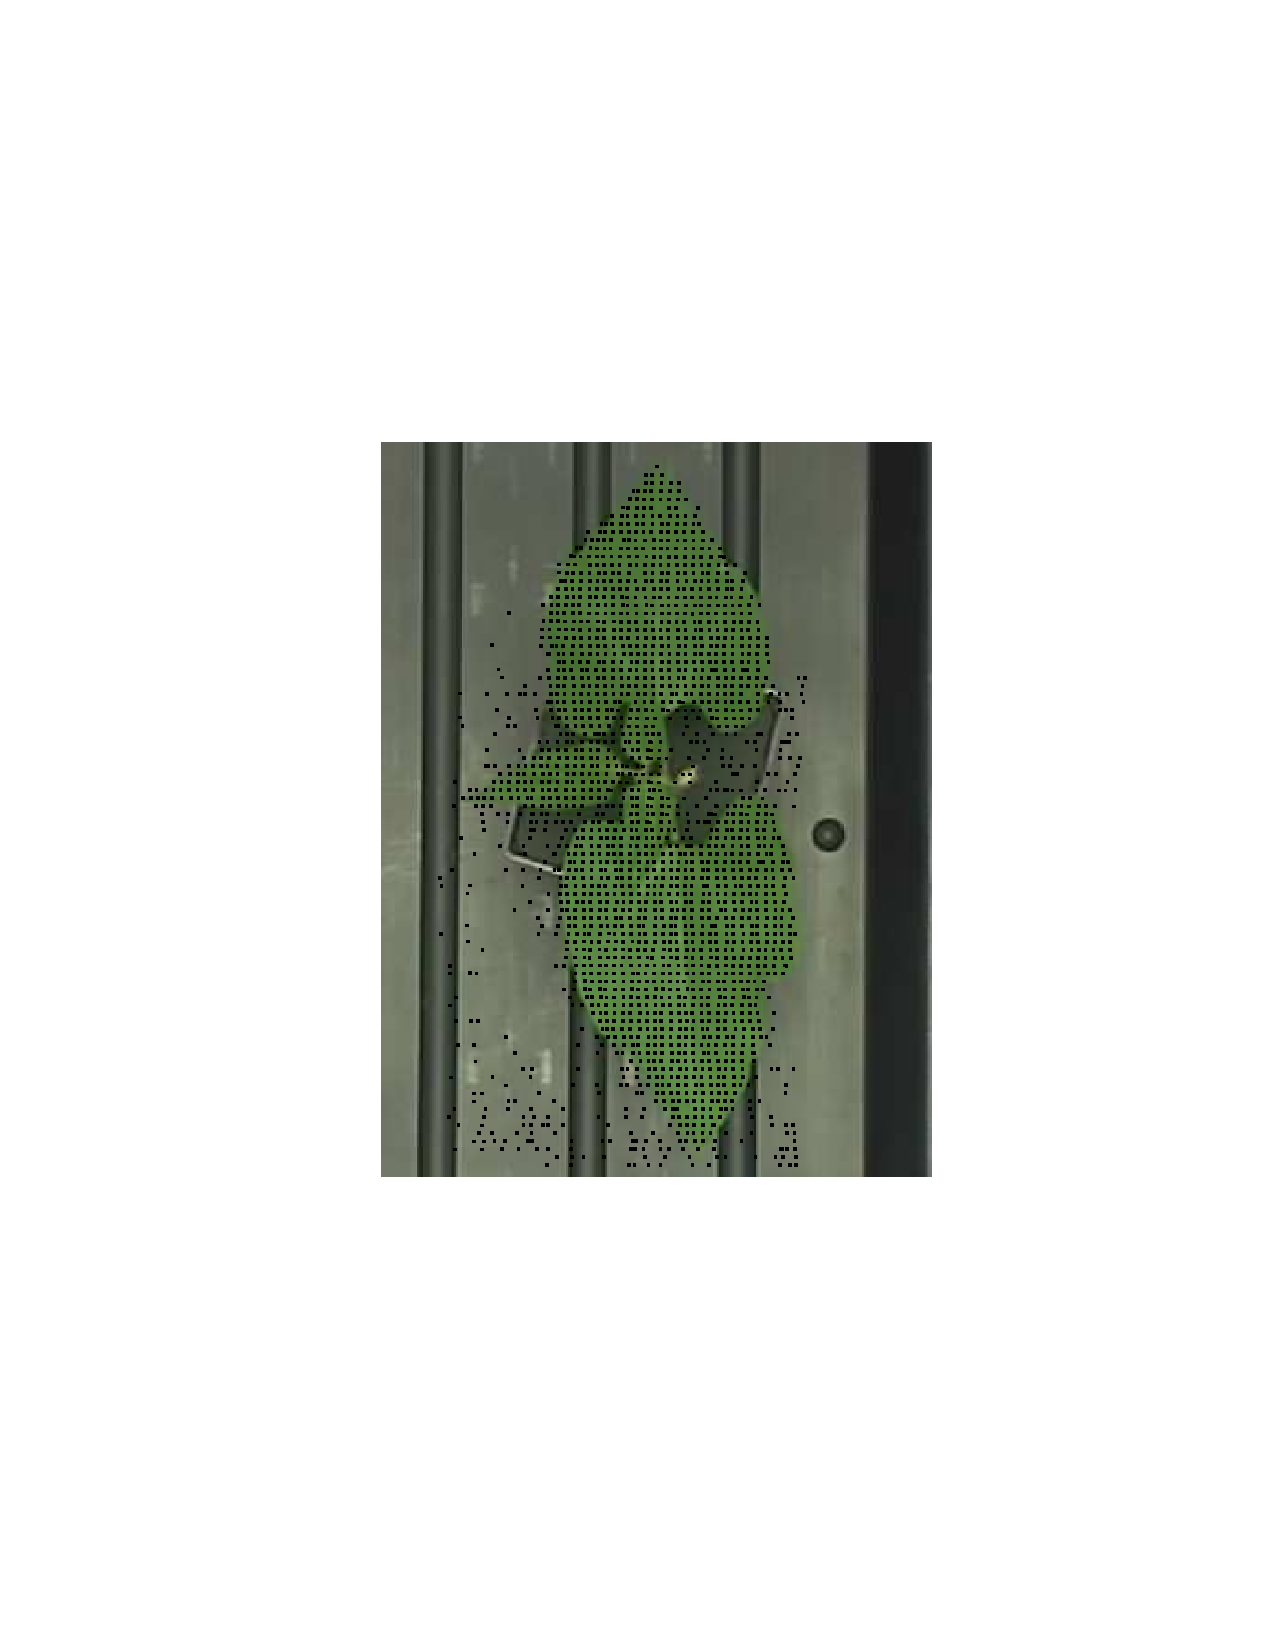
\includegraphics[width=0.65\linewidth,trim=175 220 162 180, clip,angle=-90,origin=c]{Figures/DepthOnBeanRGB} \vspace{-10mm} \\
  ($b$)\\
\end{tabular}
\caption{($a$)A plot of the three cameras showing their relative configuration and fields of view as obtained through calibration.  Units are in $mm$, apart from the size of the images which are scaled and plotted at equal resolution.  The optical center of the color camera (left-most) defines the world coordinate system.  Close to it is the depth camera having much lower resolution.  The right-most camera is the combined fluorescent and IR camera. ($b$) $3$D points from the depth camera are projected along their rays into the world coordinates and then projected into the color and fluorescent camera images.  This shows the projection into the color image (with $90^{\circ}$ rotation for economical use of space).  Only points in a rectangular region around the plant in the depth image are selected, and these are further filtered by eliminating points with high standard deviation.  An algorithm requiring only $3$D points on the plant could select only those that fall on the leaf pixels.}
\label{fig:CameraConfiguration}
\end{figure}

The imagery data were collected once every hour.
These include the fluorescent image, the IR reflectance image with the same camera, the color image, the $3$D depth and a confidence image.
The $3$D depth image is built from the depth sensor by transforming the points into the world coordinates and is expressed in the unit of $mm$.
The confidence image is the standard deviation of the depth pixels.
This is useful for identifying pixels at depth discontinuities that are unreliably detected and result in large standard deviations.


\begin{figure}
\centering
  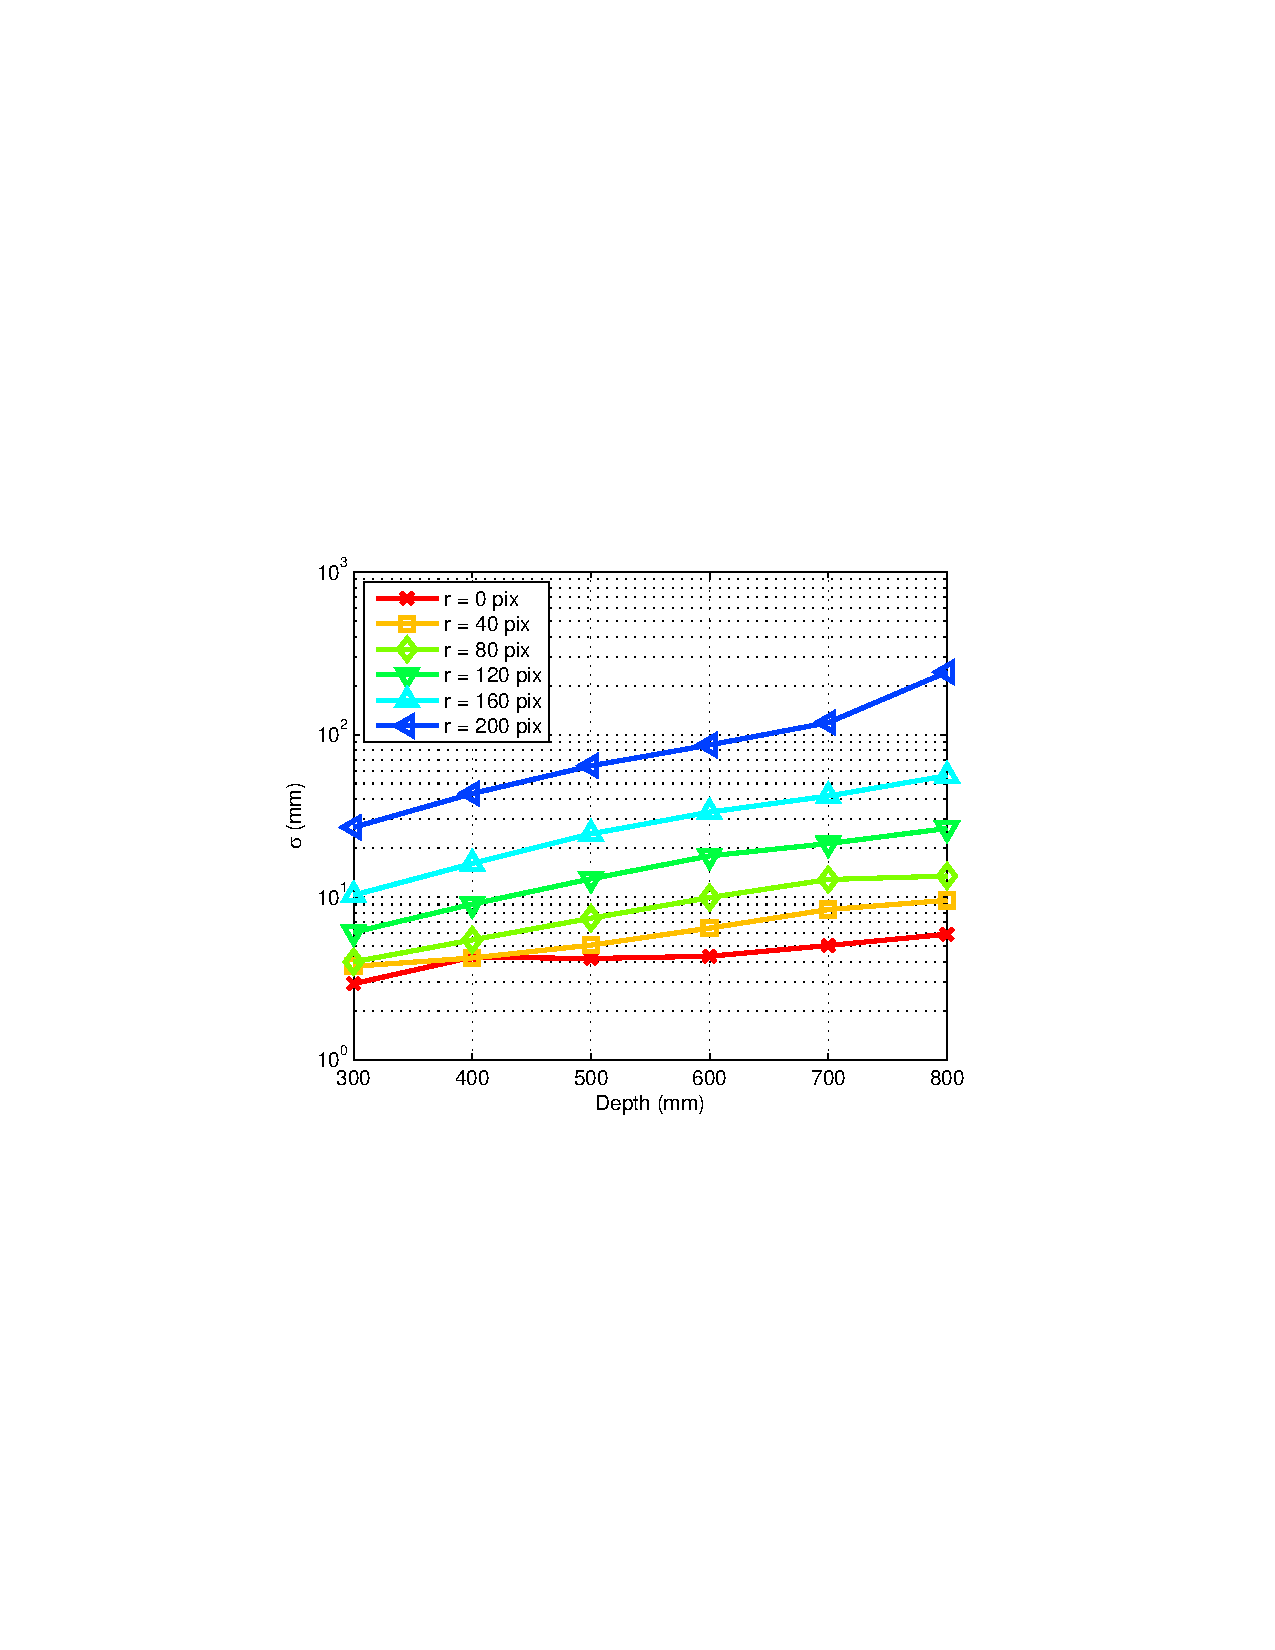
\includegraphics[height=5.9cm,trim=110 250 60 260,clip]{Figures/SigmaRadius} \\
\caption{Noise analysis for a depth camera obtained by imaging a flat surface at various depths.  We found that the standard deviation, $\sigma_I(d,r)$ from Eq. (\ref{eq:sigma}) of the pixel depth measurements had a large dependency on both the target depth, $d$, and the pixel radius, $r$, from the image center, and these are plotted.  A radius of $0$ pixels is the image center, and of $200$ pixels corresponds to the corners of the depth camera, which can be seen to have far larger standard deviation than at the image center for the same depth. }
\label{fig:Noise}
\end{figure}

